
\section{Problem 1}
%
\begin{wrapfigure}{r}{0.4\textwidth}
    \begin{center}
        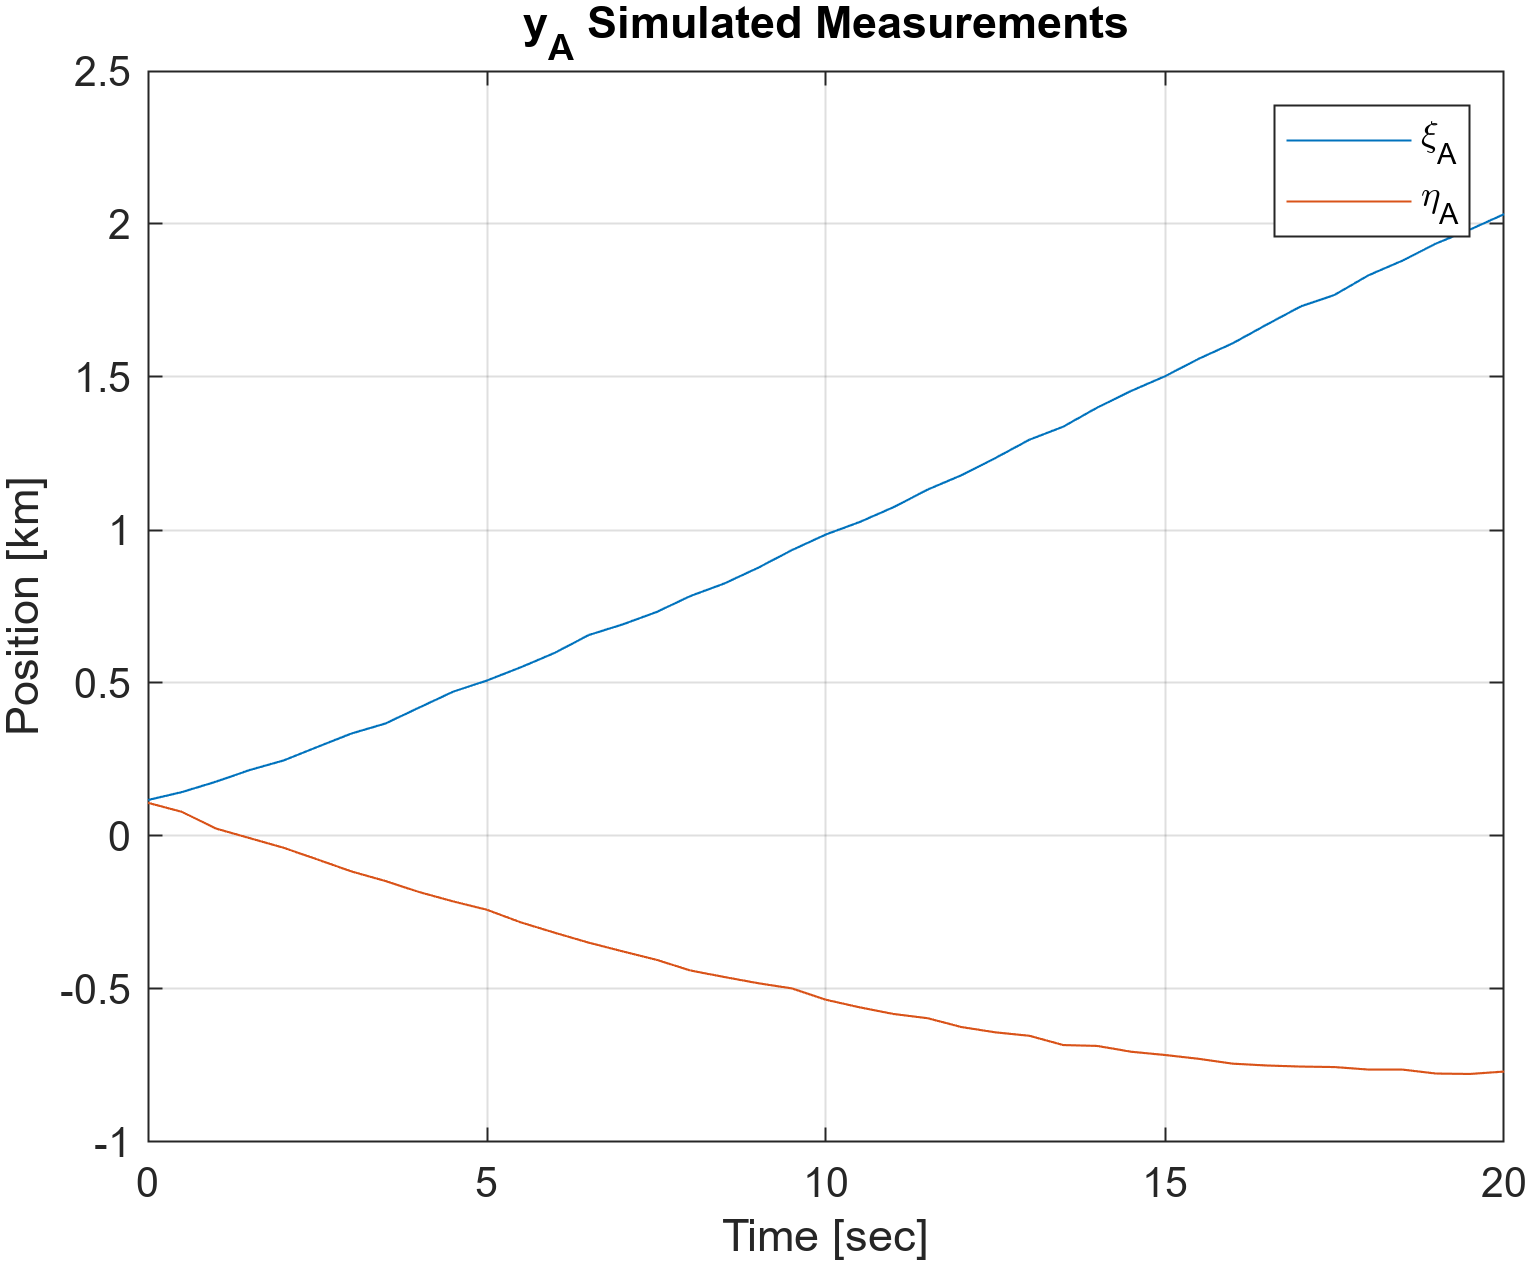
\includegraphics[width=0.8\linewidth]{figs/p2pa.png}
    \end{center}
    \caption{Wrapfigure environment}
\end{wrapfigure}
%
\lipsum[26]
\lipsum[55]
%
\subsection{Part A}
\begin{remark}[test]
    \lipsum[55]
\end{remark}
%
\lipsum[23]
%
\begin{definition}[test]
    \lipsum[44]
\end{definition}
%
\lipsum[32]
%
\subsection{Part B}
%
\begin{figure}[h!tbp]
    \centering
    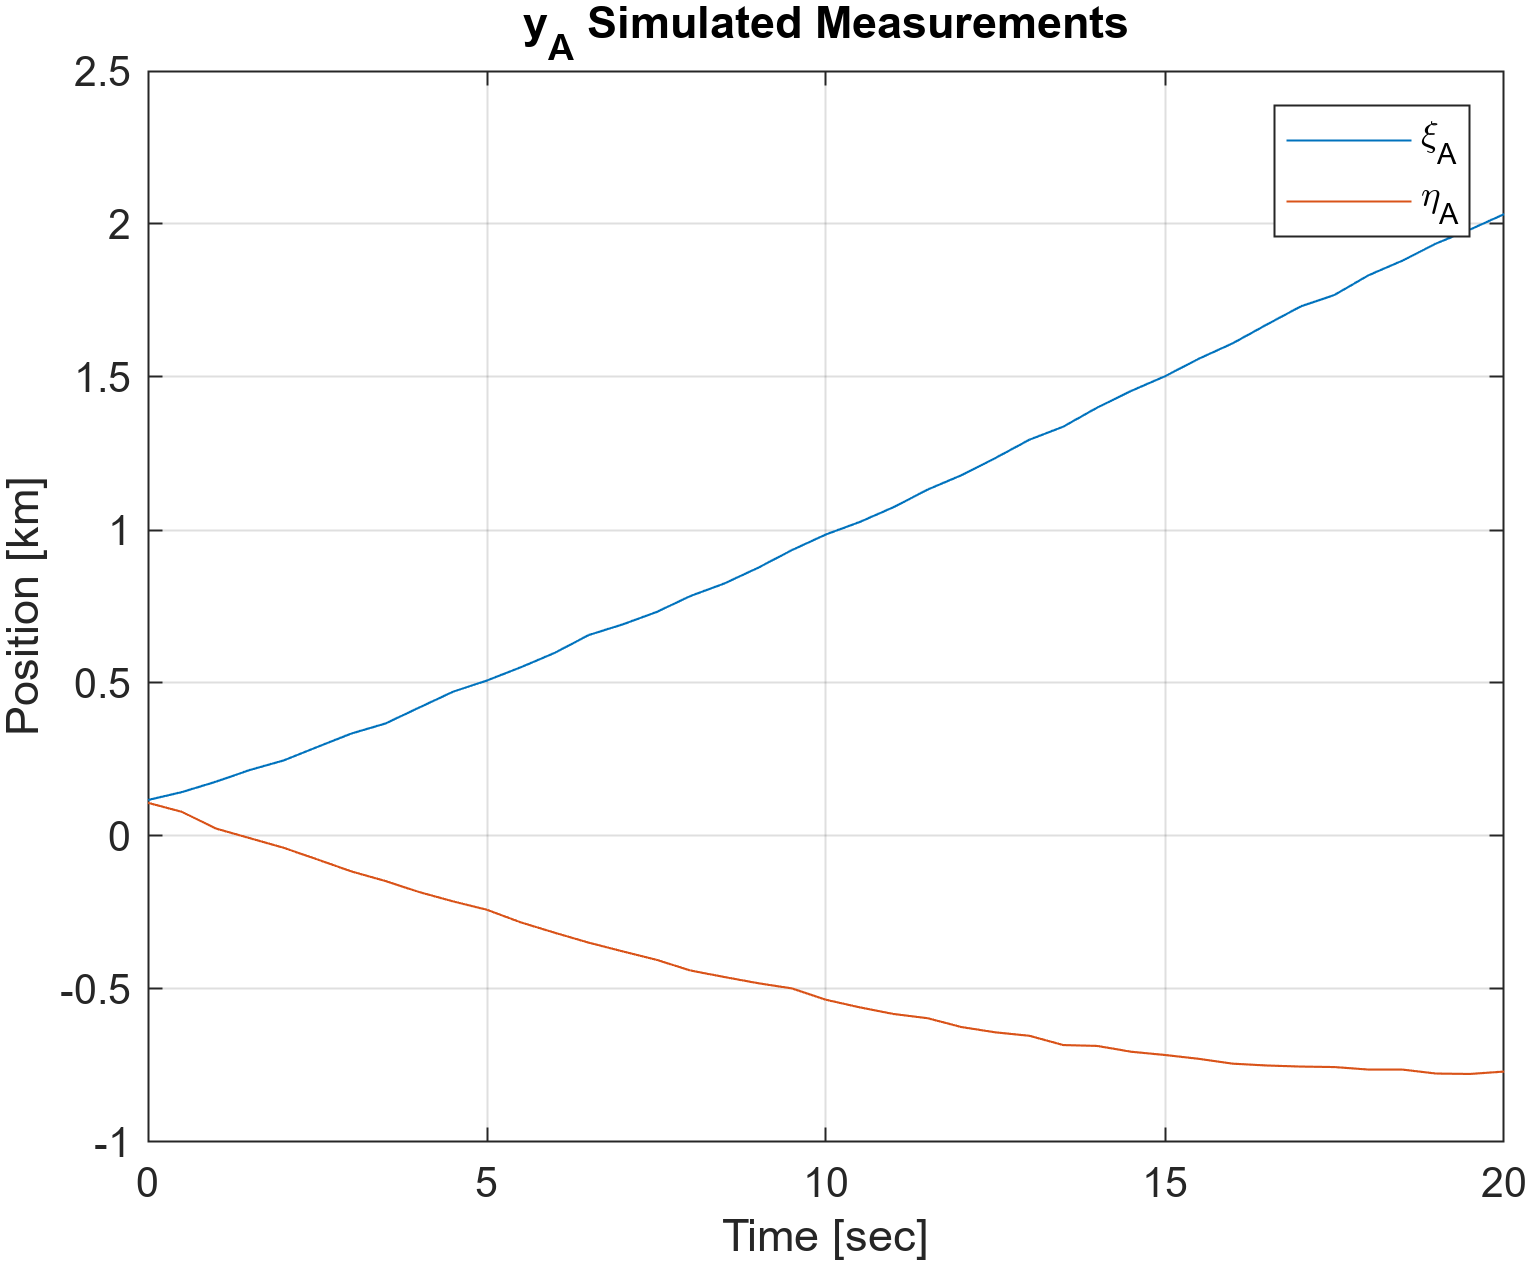
\includegraphics[width=0.6\textwidth]{figs/p2pa.png}
    \caption{Figure environment}
    \label{fig:p2_a}
\end{figure}
%
\begin{theorem}[test]
    \lipsum[2]
\end{theorem}
%
\lipsum[34]
%
\begin{eg}[test]
    \lipsum[36]
\end{eg}
%
\subsection{Code Example}
\inputminted{python3}{code/code_ex.py}